% =============================================================================
%  ME319 Assignment 2 - Guardian predictive turret control - IEEE conference paper
%  Compile with pdflatex (Overleaf: upload the whole "paper" folder, main.tex as
%  the main document). Figures: figures/*.pdf, generated by make_paper_figures.m.
%  Table rows: tables/*_rows.tex, generated by make_paper_figures.m (edit table
%  captions/headers here; re-running the script overwrites only the row files).
%  Items that you MUST complete are marked \todo{...} and print in red.
% =============================================================================
\documentclass[conference]{IEEEtran}
\usepackage{amsmath,amssymb}
\usepackage{graphicx}
\usepackage{booktabs}
\usepackage{array}
\usepackage{xcolor}
\usepackage{cite}
\usepackage{tikz}
\usetikzlibrary{positioning,arrows.meta,calc}
\usepackage[hidelinks]{hyperref}

\newcommand{\todo}[1]{\textcolor{red}{[TODO: #1]}}
\newcommand{\vect}[1]{\mathbf{#1}}
\newcommand{\Tp}{T_p}
% Loads generated table rows inside a tabular. (Plain \input fails there with
% "Misplaced \noalign" before \bottomrule; the TeX primitive works.)
\newcommand{\inputrows}[1]{\csname @@input\endcsname #1 }

% Compact spacing around floats and display equations (keeps the paper within
% the 6-page limit without removing content; delete this block to restore the
% IEEEtran defaults).
\setlength{\textfloatsep}{8pt plus 2pt minus 2pt}
\setlength{\floatsep}{6pt plus 2pt minus 2pt}
\setlength{\dbltextfloatsep}{8pt plus 2pt minus 2pt}
\setlength{\dblfloatsep}{6pt plus 2pt minus 2pt}
\setlength{\abovecaptionskip}{3pt}
\AtBeginDocument{%
  \setlength{\abovedisplayskip}{4pt plus 1pt minus 1pt}%
  \setlength{\belowdisplayskip}{4pt plus 1pt minus 1pt}%
  \setlength{\abovedisplayshortskip}{2pt plus 1pt}%
  \setlength{\belowdisplayshortskip}{2pt plus 1pt}}

\begin{document}

\title{Delay-Matched Predictive Fire Control of a\\Laser-Turret Elevation Axis Against a Maneuvering Aerial Target}

\author{\IEEEauthorblockN{Kushagra Kushwaha (24B2191) and Khushi Aggarwal (24B2171)}
\IEEEauthorblockA{Department of Mechanical Engineering, IIT Bombay\\
ME319 Control Systems, Autumn 2026 --- Assignment 2\\
Code: \todo{https://github.com/\textless user\textgreater/\textless repo\textgreater}}}

\maketitle

% -----------------------------------------------------------------------------
\begin{abstract}
A predictive feedback controller is designed for the elevation axis of a laser
point-defense turret engaging a maneuvering, intermittently observable target.
An extended Kalman filter with a Singer acceleration model estimates the target
state from noisy 20\,Hz polar radar measurements and predicts it over the
prescribed horizon $\Tp=0.5$\,s. Because the laser time of flight is negligible,
a hit requires the beam to point at the \emph{current} target position, not at the
predicted one. We therefore design a first-order lag compensator analytically so
that the closed loop $T(s)$ matches $e^{-s\Tp}$ to second order: the loop lag
cancels the prediction lead, giving zero pointing error for constant angular
velocity and acceleration. The design has a 65.4$^\circ$ phase margin and a
38.0\,dB gain margin, with dominant poles at $-2.02\pm j2.01$. A fire-control
law fires only when the laser has recharged and the beam passes within the
engagement radius with a $2\sigma$ confidence margin. In simulation, all nine
deterministic scenarios and 50 random admissible engagements were intercepted,
with a median first-interception time of 1.17\,s and 99.5\,\% of pulses within
the 2\,m engagement radius.
\end{abstract}

\begin{IEEEkeywords}
fire control, target tracking, Singer model, extended Kalman filter, lag compensator, root locus, Routh--Hurwitz.
\end{IEEEkeywords}

% -----------------------------------------------------------------------------
\section{Introduction}
The Guardian point-defense system must direct a high-energy laser at a V-44
aerial target that maneuvers within bounded speed ($\le150$\,m/s) and
acceleration ($\le20$\,m/s$^2$) limits and can be invisible to radar for up to
0.5\,s. The problem is posed in the elevation plane. A co-located radar measures
range $r$ and elevation $\theta_m$ at 20\,Hz with $\sigma_r=1$\,m and
$\sigma_\theta=0.02^\circ$. A dc-motor drive with a 100:1 reduction moves the turret,
whose elevation is limited to $[-10^\circ,85^\circ]$. Laser pulses need at least
1\,s between them, and a pulse is successful if the beam passes within
$R_{eng}=2$\,m of the target.

\textit{Objectives:} (i) estimate the target state from noisy and intermittent
measurements; (ii) predict it $\Tp=0.5$\,s ahead and form an elevation
reference; (iii) design an LTI compensator $G_c(s)$, by analytical methods, for
the turret plant $G_p(s)$; and (iv) decide when to fire so that the first hit
comes early and pulses are accurate.

\textit{Key observation and approach:} the WW-II predictors that inspired this
problem aimed a slow projectile at the target's future position. Here the laser
arrives instantly, so the beam must coincide with the target \emph{at the firing
instant}. A loop that tracks the predicted reference perfectly would point
$\Tp\dot\theta$ ahead of the target, which is tens of metres. We instead use the
prediction horizon to cancel the lag of a deliberately gentle feedback loop
(Section~\ref{sec:design}). The principal assumptions are: a rigid, lossless
gearbox; a balanced trunnion (no gravity torque); turret initially stowed at
$\theta=0$; no motor-voltage limit (none is specified); and a
turret/radar origin with $x$ the ground range and $y$ the altitude.

% -----------------------------------------------------------------------------
\section{System Architecture and Design}
Fig.~\ref{fig:schematic} shows the engagement geometry and Fig.~\ref{fig:block}
the predictive-feedback architecture. Each radar sample updates an EKF whose
state is propagated, at every control step (1\,kHz), to two epochs: the present
time $t$, used by the fire logic, and $t+\Tp$, used to form the reference
$\theta_{ref}$. The compensator drives the motor voltage $V_m$ from
$e=\theta_{ref}-\theta$. The fire logic compares the beam with the estimated
current target position and its covariance, and issues a single pulse (a 0$\to$1
edge of \texttt{fire\_cmd}) when the recharge and radius conditions are met.
The design rests on four decisions, each justified in the following sections:

\begin{enumerate}
\item \emph{Cartesian Singer EKF with a polar measurement.} Bounded, smooth
maneuvers are modelled as exponentially correlated acceleration; the radar is
used directly, without converted measurements.
\item \emph{Prediction from the last update time.} The horizon $t-t_k+\Tp$ also
accounts for the age of the 20\,Hz sample and for radar loss.
\item \emph{Delay-matched lag compensator.} $G_c(s)=K_c/(\tau_c s+1)$, with $K_c$
and $\tau_c$ obtained in closed form from the plant and $\Tp$.
\item \emph{Probabilistic fire gate.} The beam must be within $R_{eng}$ with a
$2\sigma$ margin, and the laser must have recharged.
\end{enumerate}

\begin{figure}[!t]
\centering
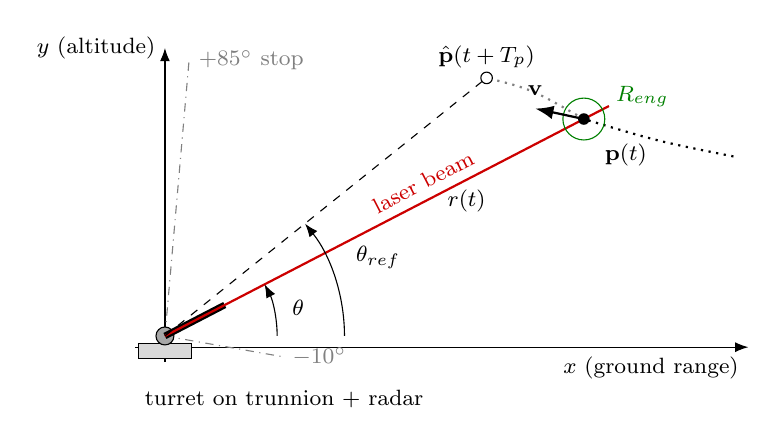
\begin{tikzpicture}[>=Latex, scale=0.95, every node/.style={font=\footnotesize}]
  \draw[->] (-0.4,0) -- (7.8,0) node[below left] {$x$ (ground range)};
  \draw[->] (0,-0.2) -- (0,4.0) node[left] {$y$ (altitude)};
  % mechanical limits
  \draw[gray, dash dot] (0,0.15) -- ++(85:3.7) node[right] {$+85^\circ$ stop};
  \draw[gray, dash dot] (0,0.15) -- ++(-10:1.6) node[right] {$-10^\circ$};
  % turret on trunnion
  \filldraw[fill=gray!30] (-0.35,-0.15) rectangle (0.35,0.05);
  \filldraw[fill=gray!70] (0,0.15) circle (0.12);
  \draw[line width=2.4pt] (0,0.15) -- ++(27.4:0.9);
  % target, trajectory, predicted point
  \coordinate (O) at (0,0.15);
  \coordinate (T) at (5.6,3.05);
  \coordinate (P) at (4.3,3.6);
  \draw[dotted, thick] (7.6,2.55) .. controls (6.6,2.75) .. (T);
  \draw[dotted, thick, gray] (T) .. controls (4.9,3.45) .. (P);
  \draw[red!80!black, thick] (O) -- ($(O)!1.06!(T)$)
     node[pos=0.6, above, sloped, text=red!80!black] {laser beam};
  \draw[dashed] (O) -- (P);
  \fill (T) circle (2.2pt);
  \draw[green!50!black] (T) circle (0.28);
  \node[green!50!black, anchor=west] at ($(T)+(0.3,0.3)$) {$R_{eng}$};
  \draw[->, thick] (T) -- ++(-0.65,0.14) node[above=1pt] {$\vect v$};
  \filldraw[fill=white] (P) circle (2.2pt) node[above] {$\hat{\vect p}(t+\Tp)$};
  \node[anchor=north west] at ($(T)+(0.15,-0.2)$) {$\vect p(t)$};
  % angles and range
  \draw[->] (1.5,0.15) arc[start angle=0, end angle=27.4, radius=1.5];
  \node at (1.78,0.52) {$\theta$};
  \draw[->] (2.4,0.15) arc[start angle=0, end angle=38.7, radius=2.4];
  \node at (2.85,1.2) {$\theta_{ref}$};
  \node[below, sloped] at ($(O)!0.72!(T)$) {$r(t)$};
  \node[anchor=north west] at (-0.4,-0.45) {turret on trunnion + radar};
\end{tikzpicture}
\caption{Elevation-plane engagement geometry. The reference points at the
predicted position $\hat{\vect p}(t+\Tp)$. The delay-matched loop makes the
turret, and hence the beam, lag that reference so that it lies on the current
position $\vect p(t)$.}
\label{fig:schematic}
\end{figure}

\begin{figure*}[!t]
\centering
\resizebox{\textwidth}{!}{%
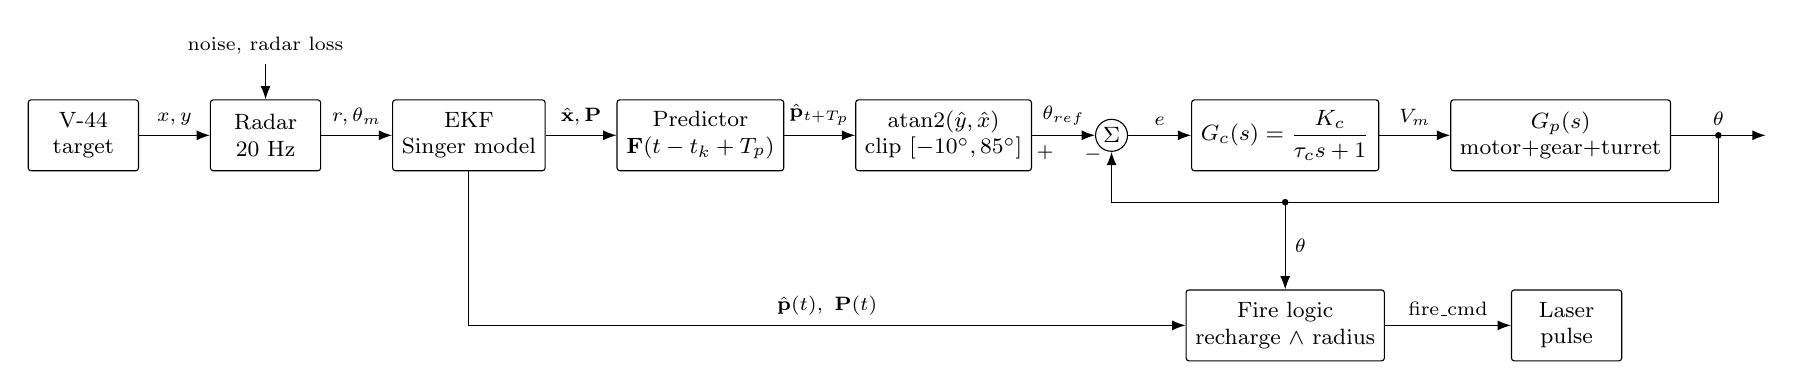
\begin{tikzpicture}[>=Latex, node distance=4mm and 9mm,
  blk/.style={draw, rounded corners=1pt, minimum height=9mm, minimum width=14mm, align=center, font=\footnotesize},
  sum/.style={draw, circle, inner sep=1.2pt, font=\footnotesize},
  lbl/.style={font=\scriptsize}]
  \node[blk] (tgt) {V-44\\target};
  \node[blk, right=of tgt] (rad) {Radar\\20 Hz};
  \node[blk, right=of rad] (ekf) {EKF\\Singer model};
  \node[blk, right=of ekf] (pred) {Predictor\\$\vect F(t-t_k+T_p)$};
  \node[blk, right=of pred] (ref) {$\mathrm{atan2}(\hat y,\hat x)$\\clip $[-10^\circ,85^\circ]$};
  \node[sum, right=8mm of ref] (sum) {$\Sigma$};
  \node[blk, right=8mm of sum] (gc) {$G_c(s)=\dfrac{K_c}{\tau_c s+1}$};
  \node[blk, right=of gc] (gp) {$G_p(s)$\\motor+gear+turret};
  \coordinate[right=12mm of gp] (out);
  \node[blk, below=15mm of gc] (fire) {Fire logic\\recharge $\wedge$ radius};
  \node[blk, right=16mm of fire] (laser) {Laser\\pulse};
  \draw[->] (tgt) -- node[above, lbl] {$x,y$} (rad);
  \draw[->] (rad) -- node[above, lbl] {$r,\theta_m$} (ekf);
  \draw[<-] (rad.north) -- ++(0,0.45) node[above, lbl] {noise, radar loss};
  \draw[->] (ekf) -- node[above, lbl] {$\hat{\vect x},\vect P$} (pred);
  \draw[->] (pred) -- node[above, lbl] {$\hat{\vect p}_{t+T_p}$} (ref);
  \draw[->] (ref) -- node[above, lbl] {$\theta_{ref}$} node[below left, lbl] {$+$} (sum);
  \draw[->] (sum) -- node[above, lbl] {$e$} (gc);
  \draw[->] (gc) -- node[above, lbl] {$V_m$} (gp);
  \draw[->] (gp) -- node[above, lbl] {$\theta$} (out);
  \coordinate (fb) at ($(gp.east)!0.5!(out)$);
  \coordinate (fbd) at ($(fb)+(0,-0.85)$);
  \fill (fb) circle (1.2pt);
  \draw[->] (fb) -- (fbd) -| node[pos=0.97, left, lbl] {$-$} (sum.south);
  \fill (fbd -| fire.north) circle (1.2pt);
  \draw[->] (fbd -| fire.north) -- node[right, lbl] {$\theta$} (fire.north);
  \draw[->] (ekf.south) |- node[pos=0.75, above, lbl] {$\hat{\vect p}(t),\ \vect P(t)$} (fire.west);
  \draw[->] (fire) -- node[above, lbl] {fire\_cmd} (laser);
\end{tikzpicture}}
\caption{Predictive-feedback architecture (closed-loop block diagram). The
estimator and predictor form the reference; the LTI loop $G_cG_p$ positions the
turret; the fire logic issues pulses using the current estimate and its
covariance.}
\label{fig:block}
\end{figure*}

% -----------------------------------------------------------------------------
\section{Mathematical Modeling}
\subsection{Turret Elevation Plant}
\label{sec:plant}
Let $i$ be the armature current, $\omega_m=N\dot\theta$ the motor speed and
$N=100$. Kirchhoff's voltage law and Newton's law, with the rotor inertia
reflected through the gear ($J_{eq}=J_{turret}+N^2J_m=3200$\,kg\,m$^2$), give
\begin{align}
L_m\,\frac{di}{dt} &= V_m - R_m i - K_e N\dot\theta, \label{eq:elec}\\
J_{eq}\,\ddot\theta &= N K_t i - b\,\dot\theta. \label{eq:mech}
\end{align}
These equations are linear, so the small-perturbation model is exact away from
the mechanical stops. Taking Laplace transforms gives
\begin{equation}
G_p(s)=\frac{\Theta(s)}{V_m(s)}=\frac{K_N}{s\,D(s)},\qquad
D(s)=d_2s^2+d_1s+d_0,
\label{eq:Gp}
\end{equation}
with $K_N=NK_t=1000$, $d_2=L_mJ_{eq}=320$, $d_1=L_mb+R_mJ_{eq}=3350$ and
$d_0=R_mb+N^2K_tK_e=1\,001\,500$:
\begin{equation}
G_p(s)=\frac{1000}{s\,(320s^2+3350s+1\,001\,500)}.
\end{equation}
The poles are $s=0$ and $s=-5.23\pm j55.70$ ($\omega_n=55.9$\,rad/s,
$\zeta=0.094$). The back-emf term $N^2K_tK_e$ dominates $d_0$, so below the
resonance the drive behaves as a velocity source,
$\dot\theta\approx V_m/(NK_e)$, i.e.\ $G_p(s)\approx 9.985\times10^{-4}/s$.
The lightly damped electromechanical resonance limits the achievable bandwidth.
The hard stops are modelled by zeroing $\dot\theta$ and $\ddot\theta$ when the
drive pushes into a stop, and by clamping $\theta$ in the integrator.

\subsection{Target Model and Estimator (Singer EKF)}
For each Cartesian axis, the state is $[p,\,v,\,a]^\top$ and the Singer model
\cite{singer1970,li2003} represents a bounded maneuver as an exponentially
correlated acceleration:
\begin{equation}
\begin{aligned}
&\dot p=v,\quad \dot v=a,\quad \dot a=-\alpha a+w,\\
&E[w(t)w(\tau)]=2\alpha\sigma_m^2\,\delta(t-\tau),
\end{aligned}
\end{equation}
with $\alpha=1/\tau_m$. The full state is
$\vect x=[x\ v_x\ a_x\ y\ v_y\ a_y]^\top$. The exact discrete transition over
an interval $\Delta$ is
\begin{equation}
\vect F_1(\Delta)=\begin{bmatrix}1&\Delta&\tau_m^2\!\left(\frac{\Delta}{\tau_m}-1+e^{-\Delta/\tau_m}\right)\\
0&1&\tau_m\left(1-e^{-\Delta/\tau_m}\right)\\0&0&e^{-\Delta/\tau_m}\end{bmatrix},
\end{equation}
with $\vect F=\mathrm{diag}(\vect F_1,\vect F_1)$. The process-noise covariance
$\vect Q(\Delta)$ is computed exactly with Van Loan's method \cite{vanloan1978}:
$\exp\!\left(\begin{bmatrix}-\vect A & \vect G q\vect G^\top\\ \vect 0&\vect A^\top\end{bmatrix}\Delta\right)
=\begin{bmatrix}\cdot&\vect F^{-1}\vect Q\\ \vect 0&\vect F^\top\end{bmatrix}$.
The measurement $\vect z=[r,\ \theta_m]^\top$ is nonlinear in $\vect x$:
\begin{equation}
\vect h(\vect x)=\begin{bmatrix}\sqrt{x^2+y^2}\\ \mathrm{atan2}(y,x)\end{bmatrix},\quad
\vect R=\mathrm{diag}(\sigma_r^2,\sigma_\theta^2).
\end{equation}
The EKF \cite{barshalom2001} predicts
$\hat{\vect x}^-=\vect F\hat{\vect x}$, $\vect P^-=\vect F\vect P\vect F^\top+\vect Q$
and updates with the Jacobian
$\vect H=\partial\vect h/\partial\vect x|_{\hat{\vect x}^-}$:
\begin{equation}
\vect K=\vect P^-\vect H^\top(\vect H\vect P^-\vect H^\top+\vect R)^{-1},\quad
\hat{\vect x}=\hat{\vect x}^-+\vect K\,[\vect z-\vect h(\hat{\vect x}^-)].
\end{equation}
The angle residual is wrapped, and the Joseph form is used for $\vect P$. The
filter is initialised from the first return (position from $(r,\theta_m)$,
$\sigma_v=100$\,m/s, $\sigma_a=10$\,m/s$^2$). During radar loss no updates
occur: the state coasts on the model and $\vect P$ grows through $\vect Q$.
\emph{Why Singer:} a constant-velocity model lags every maneuver, while a
constant-acceleration model extrapolates a stale acceleration indefinitely,
which is risky during radar loss. The Singer model estimates the acceleration
but lets that estimate decay unless the measurements keep confirming it.

\subsection{Prediction Model and Elevation Reference}
With $t_k$ the time of the last update, the predicted state and the reference are
\begin{gather}
\hat{\vect x}(t+\Tp\,|\,t_k)=\vect F(t-t_k+\Tp)\,\hat{\vect x}(t_k|t_k),\\
\theta_{ref}(t)=\mathrm{sat}_{[-10^\circ,\,85^\circ]}\ \mathrm{atan2}\big(\hat y(t+\Tp),\,\hat x(t+\Tp)\big).
\end{gather}
For a well-estimated target this is the second-order Taylor predictor
$\theta_{ref}\approx\theta_t+\Tp\dot\theta_t+\tfrac12\Tp^2\ddot\theta_t$, i.e.\
$\Theta_{ref}(s)\approx e^{s\Tp}\Theta_t(s)$, with the acceleration term weighted
by the Singer decay ($\approx$0.81 for $\tau_m=1$\,s, $\Tp=0.5$\,s).

\subsection{Closed-Loop Model}
With unity feedback, $L(s)=G_c(s)G_p(s)$ and $T(s)=L/(1+L)$, the turret angle is
$\Theta=T\,\Theta_{ref}\approx T e^{s\Tp}\Theta_t$. Since the laser is
instantaneous, the quantity that matters is the \emph{pointing error}
$e_p=\theta_t-\theta$:
\begin{equation}
\frac{E_p(s)}{\Theta_t(s)}=1-T(s)\,e^{s\Tp}.
\label{eq:Ep}
\end{equation}
Equation~\eqref{eq:Ep} is the model used for controller design. Its metric
equivalent is the cross-beam distance $d\approx r\,e_p$, which must not
exceed 2\,m.

% -----------------------------------------------------------------------------
\section{Controller Design and Analysis}
\label{sec:design}
\subsection{Design Requirement: Make $T(s)$ Behave Like $e^{-s\Tp}$}
From \eqref{eq:Ep}, the ideal loop has $T(s)=e^{-s\Tp}$, i.e.\ the loop lag
exactly cancels the prediction lead. A conventional ``tight'' tracker
($T\to1$) gives $E_p\approx(1-e^{s\Tp})\Theta_t\approx-\Tp s\Theta_t$: a
steady pointing error $-\Tp\dot\theta_t$, which is 20--75\,m at the ranges and
speeds of the envelope. Requiring $T$ to approximate $e^{-s\Tp}$ only at low
frequency, where the target's angle spectrum lies, leads to a simple LTI design.

\subsection{Delay-Matched Compensator Derivation}
Choose $G_c(s)=K_c/(\tau_cs+1)$. With \eqref{eq:Gp},
\begin{equation}
\frac{1}{T(s)}=1+\frac{s(\tau_cs+1)D(s)}{K_NK_c}
=1+c_1s+c_2s^2+c_3s^3+\dots
\end{equation}
where $c_1=d_0/(K_NK_c)$, $c_2=(d_1+\tau_cd_0)/(K_NK_c)$ and
$c_3=(d_2+\tau_cd_1)/(K_NK_c)$. Matching $1/T(s)$ to
$e^{s\Tp}=1+\Tp s+\tfrac12\Tp^2s^2+\tfrac16\Tp^3s^3+\dots$ term by term gives
\begin{equation}
\boxed{K_c=\frac{d_0}{K_N\Tp}=2003\ \tfrac{\mathrm{V}}{\mathrm{rad}},\qquad
\tau_c=\frac{\Tp}{2}-\frac{d_1}{d_0}=0.2467\ \mathrm{s}.}
\end{equation}
Then $T(s)e^{s\Tp}=1+(\Tp^3/6-c_3)s^3+\dots$, so
\begin{equation}
e_p(t)\approx-\Big(\tfrac{\Tp^3}{6}-c_3\Big)\,\dddot\theta_t
=-0.0203\,\dddot\theta_t\quad(c_3=5.7\times10^{-4}).
\label{eq:resid}
\end{equation}
The predictive loop has \emph{zero pointing error for constant target angular
velocity and constant angular acceleration}; the residual is proportional to the
angular jerk. For scenario B ($A\omega\approx19$\,m/s$^3$ at $r\approx1.5$\,km,
$\dddot\theta_t\approx0.013$\,rad/s$^3$) this gives $e_p\approx0.26$\,mrad, or
0.4\,m, which is within $R_{eng}$. The gains are fixed by the plant constants
and $\Tp$ alone; no numerical tuning was used. Note that the reference-tracking
error $\theta_{ref}-\theta\approx\Tp\dot\theta_t$ is intentionally non-zero
(about 1.5$^\circ$ in Fig.~\ref{fig:caseB}).

\subsection{Error Constants}
With respect to $\theta_{ref}$ the loop is type~1, with $K_p=\infty$,
$K_v=\lim_{s\to0}sL(s)=K_NK_c/d_0=1/\Tp=2$\,s$^{-1}$ and $K_a=0$. The
steady-state ramp-tracking lag is therefore $1/K_v=\Tp$, which is exactly what
the predictor removes. Without an integrator in $G_c$, voltage saturation
cannot cause windup.

\subsection{Stability: Routh--Hurwitz}
The characteristic equation $s(\tau_cs+1)D(s)+K_NK_c=0$ is
\begin{equation}
78.93s^4+1146.3s^3+250\,375s^2+1\,001\,500s+2\,003\,000=0.
\end{equation}
The Routh array \cite{ogata} is
\begin{center}\footnotesize
\begin{tabular}{l|lll}
$s^4$ & 78.93 & 250\,375 & 2\,003\,000\\
$s^3$ & 1146.3 & 1\,001\,500 & \\
$s^2$ & $b_1=181\,415$ & 2\,003\,000 & \\
$s^1$ & $c_1=988\,844$ & & \\
$s^0$ & 2\,003\,000 & &
\end{tabular}
\end{center}
The first column has no sign change, so the closed loop is stable. Since $b_1$
does not depend on $K_c$, the $s^1$ row gives the stability range analytically:
\begin{equation}
0<K_c<K_{c,\mathrm{crit}}=\frac{b_1d_0}{a_3K_N}=1.585\times10^5\ \mathrm{V/rad},
\end{equation}
with $a_3=\tau_cd_1+d_2$. This is a gain margin of $79.1\times$ (38.0\,dB). At
$K_{c,\mathrm{crit}}$ the auxiliary equation $b_1s^2+K_NK_{c,\mathrm{crit}}=0$
gives sustained oscillation at $\omega=29.6$\,rad/s.

\subsection{Root Locus and Frequency Response}
Fig.~\ref{fig:rlocus} shows the root locus \cite{franklin} as $K_c$ is scaled. The
compensator pole ($-4.05$) and the free integrator meet and break away into the
dominant pair, which reaches $-2.02\pm j2.01$ ($\omega_n=2.85$\,rad/s,
$\zeta=0.708$) at the design gain: a near-Butterworth pair, consistent with
matching $e^{-s\Tp}$ (the second-order fit $1/(1+\Tp s+\tfrac12\Tp^2s^2)$ has
$\omega_n=\sqrt2/\Tp$, $\zeta=1/\sqrt2$). The resonant pair barely moves
($-5.24\pm j55.63$). The Bode plot (Fig.~\ref{fig:bode}) gives a phase
margin of 65.4$^\circ$ at 1.83\,rad/s and a gain margin of 38.0\,dB at
29.6\,rad/s, matching the Routh result. The resonance peak stays more than
35\,dB below 0\,dB. The closed-loop bandwidth is 2.86\,rad/s.

\begin{figure}[!t]
\centering
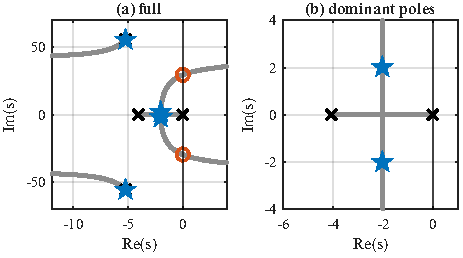
\includegraphics[width=\columnwidth]{figures/fig_rlocus.pdf}
\caption{Root locus of $G_cG_p$ versus a gain multiplier on $K_c$
($\times$ open-loop poles, $\star$ design closed-loop poles, $\circ$
imaginary-axis crossing at $79.1K_c$, $\omega=29.6$\,rad/s).}
\label{fig:rlocus}
\end{figure}

\begin{figure}[!t]
\centering
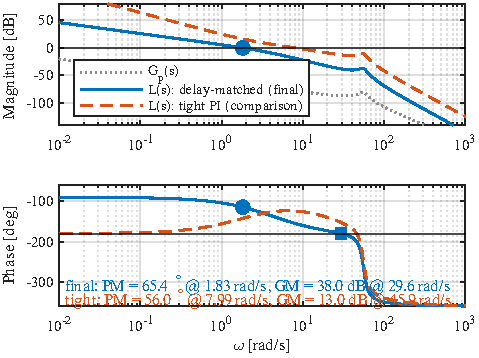
\includegraphics[width=\columnwidth]{figures/fig_bode.pdf}
\caption{Bode plot of $L(s)$ for the final delay-matched design and for the
comparison tight PI design, with margins.}
\label{fig:bode}
\end{figure}

\subsection{Transient Response}
The unit-step response (Fig.~\ref{fig:step}) has a 0.75\,s rise time, a 2.09\,s
settling time (2\,\%) and 4.3\,\% overshoot. The acquisition slew from the
stowed position overshoots slightly, so the beam sweeps across the target at
about 1.17\,s; the fire logic exploits this crossing, giving the early first
interceptions in Table~\ref{tab:cases}. A $35^\circ$ slew needs at most
795\,V, against 4.0\,kV for the tight design.

\begin{figure}[!t]
\centering
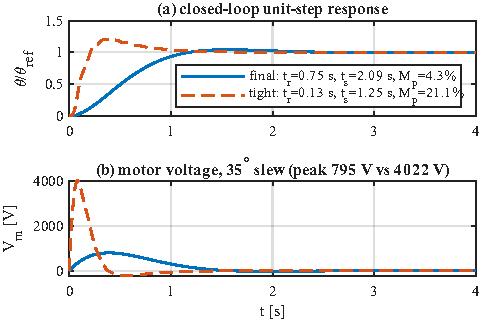
\includegraphics[width=\columnwidth]{figures/fig_step.pdf}
\caption{(a) Closed-loop step responses. (b) Motor voltage for a $35^\circ$
acquisition slew.}
\label{fig:step}
\end{figure}

\subsection{Pointing-Error Transfer, Noise and Prediction Error}
Fig.~\ref{fig:delay}(a) plots $|1-T(j\omega)e^{j\omega\Tp}|$. For the final
design it falls at 60\,dB/decade (third order, per \eqref{eq:resid}). Without
prediction, or with a tight loop plus prediction, it falls at only
20\,dB/decade, i.e.\ there is a velocity error; the high-gain type-2 loop
without prediction reaches 40\,dB/decade, leaving an acceleration error. Fig.~\ref{fig:delay}(b)
confirms this in the time domain for $\theta_t=5t+0.5t^2$\,deg: the final
design converges to zero error, the tight loop leads by $\approx\Tp\dot\theta_t$
and the unpredicted loop lags by the same amount. \emph{Measurement noise} enters
through $\theta_{ref}$. The predictor amplifies velocity-estimate noise by $\Tp$,
but $|T(j\omega)|$ is $-33$\,dB at 20\,rad/s, so the 20\,Hz radar noise reaching
the turret is strongly attenuated. The tight loop ($\omega_{BW}=13.8$\,rad/s)
passes far more noise. \emph{Prediction error} acts as an additive reference
disturbance filtered by $T(s)$. Its RMS value (Table~\ref{tab:cases}) is
1.5--3.5\,m, mostly at frequencies above the loop bandwidth, so the beam error
is smaller than the prediction error.

\begin{figure}[!t]
\centering
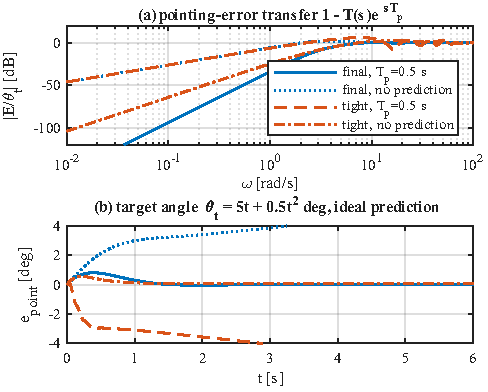
\includegraphics[width=\columnwidth]{figures/fig_delay.pdf}
\caption{Delay matching. (a) Pointing-error transfer $|1-Te^{s\Tp}|$. (b) Pointing
error for a ramp-plus-parabola target angle.}
\label{fig:delay}
\end{figure}

\subsection{Measurement Loss and Physical Limits}
During a loss of duration $t_{bo}\le0.5$\,s the reference is extrapolated over
up to $t_{bo}+\Tp\le1$\,s, and the error grows roughly as
$\tfrac12\Delta a\,(t_{bo}+\Tp)^2$ for an unmodelled acceleration change
$\Delta a$. The EKF covariance grows accordingly. The fire logic reads the
cross-beam standard deviation $\sigma_\perp$ and stops firing until the track
re-converges (Fig.~\ref{fig:caseC}(c)), which prevents wasted pulses. Because
$T(s)$ is well damped, the transient after recovery decays within about
$4/(\zeta\omega_n)\approx2$\,s. The elevation limits are handled by clipping
$\theta_{ref}$ (so the loop never commands a stop) and by modelling the hard
stops. Scenario H, where the target passes $85^\circ$, shows the expected loss
of pointing only after the stop is reached.

\subsection{Fire-Control Logic}
With beam direction $\vect u=[\cos\theta,\sin\theta]^\top$, normal
$\vect n=[-\sin\theta,\cos\theta]^\top$ and the current estimate $\hat{\vect p}(t)$
with covariance $\vect P_{pp}(t)$, the controller computes
\begin{equation}
\hat d=\begin{cases}|\vect n^\top\hat{\vect p}|,& \vect u^\top\hat{\vect p}>0\\ \|\hat{\vect p}\|,&\text{otherwise}\end{cases},\qquad
\sigma_\perp=\sqrt{\vect n^\top\vect P_{pp}\vect n}.
\end{equation}
A 0$\to$1 pulse is issued only if \emph{all} of the following hold:
(i) $t-t_{last}\ge1$\,s (recharged);
(ii) $\hat d+k_\sigma\sigma_\perp\le R_{eng}$ with $k_\sigma=2$, i.e.\
inside the radius at roughly 97.7\,\% one-sided confidence;
(iii) $\sigma_\perp\le0.75$\,m; and
(iv) the track is at least 0.25\,s old.
The simulator models the laser independently: it ignores early edges and scores
each pulse by the distance from the ray to the \emph{true} target position.

\subsection{Alternatives Considered}
Table~\ref{tab:cmp} compares four architectures on scenarios A--I.
Tracking the predicted reference tightly (2) fails, because the beam leads the
target, and so does the gentle loop without prediction (4), because the beam
lags it. A high-gain type-2 loop without prediction (3) also works, but it needs
about 5$\times$ the voltage, has a 13\,dB rather than 38\,dB gain margin, passes
more noise, intercepts later on average, and leaves out the prescribed
prediction stage. The delay-matched design (1) was therefore chosen. The PI
baseline uses standard rules ($\omega_c=8$\,rad/s, $\omega_i=\omega_c/4$,
$\omega_f=3\omega_c$) and was not optimised.

\begin{table}[!t]
\centering
\caption{Architecture comparison on scenarios A--I (same EKF and fire logic)}
\label{tab:cmp}
\footnotesize
\setlength{\tabcolsep}{3pt}
\begin{tabular}{@{}>{\raggedright\arraybackslash}p{3.1cm}ccccc@{}}
\toprule
Variant & Succ. & $\bar t_{int}$ [s] & RMS $d$ [m] & Hits & $V_{pk}$ [V]\\
\midrule
\inputrows{tables/comparison_rows.tex}
\bottomrule
\end{tabular}
\end{table}

% -----------------------------------------------------------------------------
\section{Simulation and Results}
\subsection{Setup}
The master script integrates the plant with RK4 at 1\,kHz (zero-order-hold
voltage). It calls the prescribed \texttt{target\_motion\_generator},
\texttt{turret\_controller} and \texttt{turret\_plant} functions at every step;
the radar returns new samples at 20\,Hz. The compensator is discretised
exactly (ZOH) at the actual call interval, so the controller is independent of
the evaluation rate. Scenarios A (nominal), B (weave in $x$ and $y$ from 1\,s)
and C (loss 1.0--1.5\,s) are the standardised cases. Cases D--I add a maneuver
during loss, high-g jinks near $a_{max}$, a fast climbing crosser, a diving
attack, a near-overhead pass reaching the $85^\circ$ stop, and a 140\,m/s
long-range target with a late loss. Every trajectory is verified
programmatically against the range, speed, acceleration and loss bounds. Each
target is a constant-velocity baseline plus analytically integrated windowed
sinusoidal accelerations, which keeps the acceleration continuous. The design
parameters are listed in Table~\ref{tab:params}.

\begin{table}[!t]
\centering
\caption{Design parameters (single set for all cases)}
\label{tab:params}
\footnotesize
\begin{tabular}{@{}lll@{}}
\toprule
Block & Parameter & Value \\
\midrule
Compensator & $K_c$, $\tau_c$ & 2003 V/rad, 0.2467 s (analytical)\\
Predictor & $\Tp$ & 0.50 s (prescribed)\\
EKF & $\sigma_m$, $\tau_m$ & 8 m/s$^2$, 1.0 s (Table~\ref{tab:sens})\\
EKF & $\sigma_{v0}$, $\sigma_{a0}$ & 100 m/s, 10 m/s$^2$\\
Fire logic & $k_\sigma$, $\sigma_{max}$, min.\ age & 2, 0.75 m, 0.25 s\\
Simulation & $\Delta t$, $\theta(0)$, $V_{max}$ & 1 ms, $0^\circ$, none\\
\bottomrule
\end{tabular}
\end{table}

\subsection{Results}
Figs.~\ref{fig:caseB}--\ref{fig:estB} and Table~\ref{tab:cases} summarise the
results. In scenario B the turret follows $\theta_t$, not $\theta_{ref}$, and
every pulse lies inside $R_{eng}$, which confirms the delay-matching analysis.
The slow $\pm2$\,m oscillation of the pointing error follows the weave and is
caused by the acceleration-estimation lag, consistent with \eqref{eq:resid}. In
scenario C the slew crossing at 1.17\,s occurs during the radar loss. The fire
logic correctly withholds the pulse because $\sigma_\perp$ exceeds the gate,
so the first hit comes after re-convergence (2.61\,s). The position estimate
stays within its $2\sigma$ bounds throughout. The velocity error stays within
about $\pm5$\,m/s during the weave, and the 0.5\,s prediction error stays
within about $\pm5$\,m. All nine cases are intercepted, with 72 of 72 pulses
inside $R_{eng}$ and peak voltage at most 1.26\,kV (during the largest
acquisition slew).

\begin{figure}[!t]
\centering
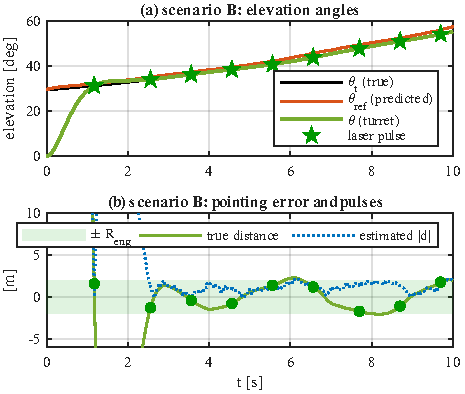
\includegraphics[width=\columnwidth]{figures/fig_caseB.pdf}
\caption{Scenario B (maneuvering target). (a) True, reference and turret
elevation; stars mark pulses. (b) True beam--target distance, estimated
distance and pulse outcomes (green: hit).}
\label{fig:caseB}
\end{figure}

\begin{figure}[!t]
\centering
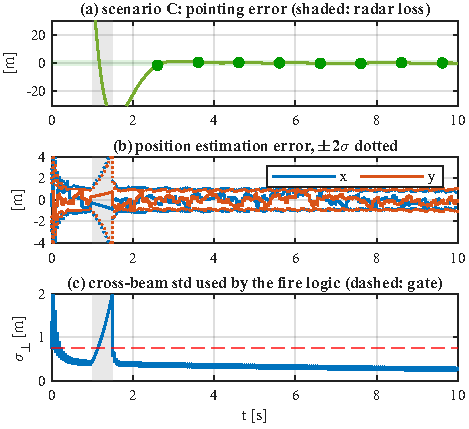
\includegraphics[width=\columnwidth]{figures/fig_caseC.pdf}
\caption{Scenario C (radar loss 1.0--1.5\,s, shaded). (a) Pointing error and
pulses. (b) Position estimation error with $\pm2\sigma$ bounds. (c) Cross-beam
standard deviation and the fire gate.}
\label{fig:caseC}
\end{figure}

\begin{figure}[!t]
\centering
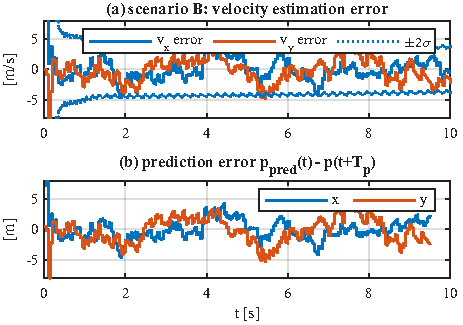
\includegraphics[width=\columnwidth]{figures/fig_estB.pdf}
\caption{Scenario B estimator performance. (a) Velocity estimation error. (b)
Error of the 0.5\,s prediction against the true future position.}
\label{fig:estB}
\end{figure}

\begin{table*}[!t]
\centering
\caption{Performance of the finalized design ($d$: true beam--target distance,
$t\ge3$\,s; estimation and prediction errors for $t\ge1$\,s; $t_{rec}$: time
after radar loss until $|d|\le R_{eng}$)}
\label{tab:cases}
\footnotesize
\begin{tabular}{@{}lccccccccc@{}}
\toprule
Case & $t_{int}$ [s] & Hits/pulses & mean miss [m] & RMS $d$ [m] & RMS $\tilde{\vect p}$ [m] & RMS $\tilde{\vect p}_{t+T_p}$ [m] & beam in $R_{eng}$ [\%] & $t_{rec}$ [s] & $V_{pk}$ [V]\\
\midrule
\inputrows{tables/cases_rows.tex}
\bottomrule
\end{tabular}
\end{table*}

\subsection{Estimator Parameter Selection}
The Singer parameters were the only quantities selected numerically, as the
assignment permits for the estimator. A $4\times3$ grid was evaluated on 20
random admissible engagements whose seeds are disjoint from the evaluation set
(Table~\ref{tab:sens}). All settings intercepted every case. Larger $\sigma_m$
improves maneuver tracking but increases prediction noise, and shorter
$\tau_m$ reduces acceleration extrapolation. The pair $\sigma_m=8$\,m/s$^2$,
$\tau_m=1$\,s gives the best overall balance. The initial guess was
$\tau_m=2$\,s.

\begin{table}[!t]
\centering
\caption{Estimator sensitivity on tuning cases: time with beam in $R_{eng}$ [\%] / mean pulse miss [m]}
\label{tab:sens}
\footnotesize
\setlength{\tabcolsep}{4pt}
\begin{tabular}{@{}lccc@{}}
\toprule
$\sigma_m$ [m/s$^2$] & $\tau_m=1$ s & $\tau_m=2$ s & $\tau_m=4$ s\\
\midrule
\inputrows{tables/sensitivity_rows.tex}
\bottomrule
\end{tabular}
\end{table}

% -----------------------------------------------------------------------------
\section{Final Evaluation}
\textit{Generalization study.} The finalized design (unchanged, no retuning)
was evaluated on 50 random admissible engagements, generated independently of
the design scenarios and of the estimator tuning cases. Each has a random initial position and inbound velocity, one or two
smooth maneuver components per axis with random amplitude, frequency, duration
and onset; 44 of the 50 cases also include a radar loss of 0.1--0.5\,s
starting between 1 and 7\,s. Targets are kept inside the turret's reachable elevation.
All 50 cases were intercepted (Fig.~\ref{fig:mc}). The median first
interception was 1.17\,s (90th percentile 1.18\,s, worst 2.60\,s, a case with
radar loss during acquisition). 99.5\,\% of pulses were within $R_{eng}$ and
the mean RMS pointing error was 0.76\,m, indicating consistent performance
across maneuver types.

\begin{figure}[!t]
\centering
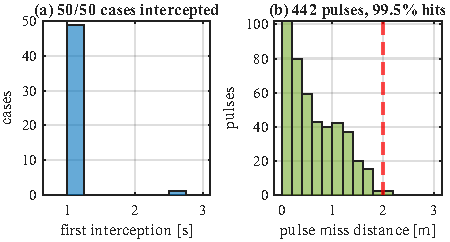
\includegraphics[width=\columnwidth]{figures/fig_mc.pdf}
\caption{Generalization over 50 random admissible engagements. (a) First
interception time. (b) Miss distance of all issued pulses (dashed: $R_{eng}$).}
\label{fig:mc}
\end{figure}

% -----------------------------------------------------------------------------
\section{Conclusions}
The prediction horizon was used to cancel, rather than to add to, the lag
of the feedback loop. Matching $T(s)$ to $e^{-s\Tp}$ to second order gives the
closed-form gains $K_c=d_0/(K_N\Tp)$ and $\tau_c=\Tp/2-d_1/d_0$. The resulting
first-order lag compensator has zero pointing error for constant angular velocity
and acceleration, large stability margins (65.4$^\circ$, 38\,dB), strong noise
and resonance attenuation, and modest voltage demand. A Singer-model EKF
provides the state and covariance, and a confidence-gated fire logic converts
them into accurate pulses. \emph{Strengths:} analytical, simple, robust to radar
loss, and independent of the call rate. \emph{Limitations:} the residual error
grows with angular jerk (aggressive close-range jinks); acquisition is limited by
the low bandwidth (about 2\,s settling); the design assumes the plant parameters
are exact (a change in $d_0$ shifts $K_v$ and hence the matched lag); no voltage
limit was imposed; and targets beyond the $85^\circ$ stop cannot be engaged. The
factors that most affect performance are the quality of the acceleration
estimate during maneuvers and the duration and timing of radar loss.

% -----------------------------------------------------------------------------
\begin{thebibliography}{9}
\bibitem{singer1970} R.~A. Singer, ``Estimating optimal tracking filter performance for manned maneuvering targets,'' \emph{IEEE Trans. Aerosp. Electron. Syst.}, vol.~AES-6, no.~4, pp.~473--483, 1970.
\bibitem{li2003} X.~R. Li and V.~P. Jilkov, ``Survey of maneuvering target tracking. Part I: Dynamic models,'' \emph{IEEE Trans. Aerosp. Electron. Syst.}, vol.~39, no.~4, pp.~1333--1364, 2003.
\bibitem{barshalom2001} Y.~Bar-Shalom, X.~R. Li, and T.~Kirubarajan, \emph{Estimation with Applications to Tracking and Navigation}. New York: Wiley, 2001.
\bibitem{vanloan1978} C.~F. Van~Loan, ``Computing integrals involving the matrix exponential,'' \emph{IEEE Trans. Autom. Control}, vol.~23, no.~3, pp.~395--404, 1978.
\bibitem{ogata} K.~Ogata, \emph{Modern Control Engineering}, 5th~ed. Upper Saddle River, NJ: Prentice Hall, 2010.
\bibitem{franklin} G.~F. Franklin, J.~D. Powell, and A.~Emami-Naeini, \emph{Feedback Control of Dynamic Systems}, 8th~ed. Pearson, 2019.
\end{thebibliography}

% =============================================================================
\clearpage
\section*{Appendix: Use of AI and Computational Tools}
\textit{Tools.} Claude Opus 5.5 (Anthropic), used through the Claude Code
command-line agent; MATLAB R2025b (base MATLAB only; the analysis code is
toolbox-free); LaTeX/Overleaf for typesetting.

\textit{How each tool contributed.} Claude was used to (i) interpret the
assignment and identify that the negligible laser time of flight makes the
\emph{current} pointing error the design objective; (ii) propose and derive the
delay-matched compensator; (iii) write the MATLAB implementation (prescribed
functions, master simulation, metrics, plots, Monte-Carlo, comparison and
sensitivity studies); and (iv) draft this paper. MATLAB was used for all
simulations, the frequency-domain analysis and the figures. The Routh array and
critical gain were also computed independently with a short script.

\textit{AI outputs accepted, modified or rejected.}
\begin{itemize}
\item \emph{Accepted (after verification):} the delay-matching derivation
($K_c$, $\tau_c$), verified by checking that the printed coefficients
$c_1=\Tp$ and $c_2=\Tp^2/2$ match, by the Routh--Hurwitz/Bode agreement
(38.0\,dB at 29.6\,rad/s), and by simulation; the Singer EKF formulation; and
the fire-gate structure.
\item \emph{Modified:} the Singer correlation time was changed from the initial
2\,s to 1\,s after the sensitivity study; the steady-state metric window was
moved from 2\,s to 3\,s after the step-settling time (2.09\,s) was found; random
cases were restricted to the reachable elevation range after targets beyond the
$85^\circ$ stop were seen to inflate the error metrics; a guard against
repeatedly fused held measurements was added for robustness to the evaluation
script.
\item \emph{Rejected:} the literal reading ``track the predicted reference as
tightly as possible'' (2/9 interceptions, Table~\ref{tab:cmp}); the high-gain
no-prediction loop despite its accuracy (5$\times$ voltage, smaller margins,
omits the prescribed prediction stage); and vector-PDF export of large figures.
\end{itemize}

\textit{Engineering validation.} The noise specification was confirmed as
$\sigma_\theta=0.02^\circ$ from the assignment text. Every trajectory is checked
programmatically against the envelope. The estimator was tuned only on seeds
disjoint from the evaluation seeds. All quantitative claims in this paper are
regenerated by \texttt{main\_guardian.m} and \texttt{make\_paper\_figures.m}.
\todo{In your own words, add how you personally checked the key results (e.g.\
re-deriving $G_p(s)$ and the Routh array by hand, re-running cases, varying
parameters) and which decisions you made yourself.}

\end{document}
